\section{[Nobel Literature Prize 1902] Theodor Mommsen}

``\textit{the greatest living master of the art of historical writing, with
  special reference to his monumental work A History of Rome}''

“\textit{历史写作最伟大的大师,尤其是其巨作《罗马史》}”

\subsection{罗马史}

\begin{figure}[H]
\centering
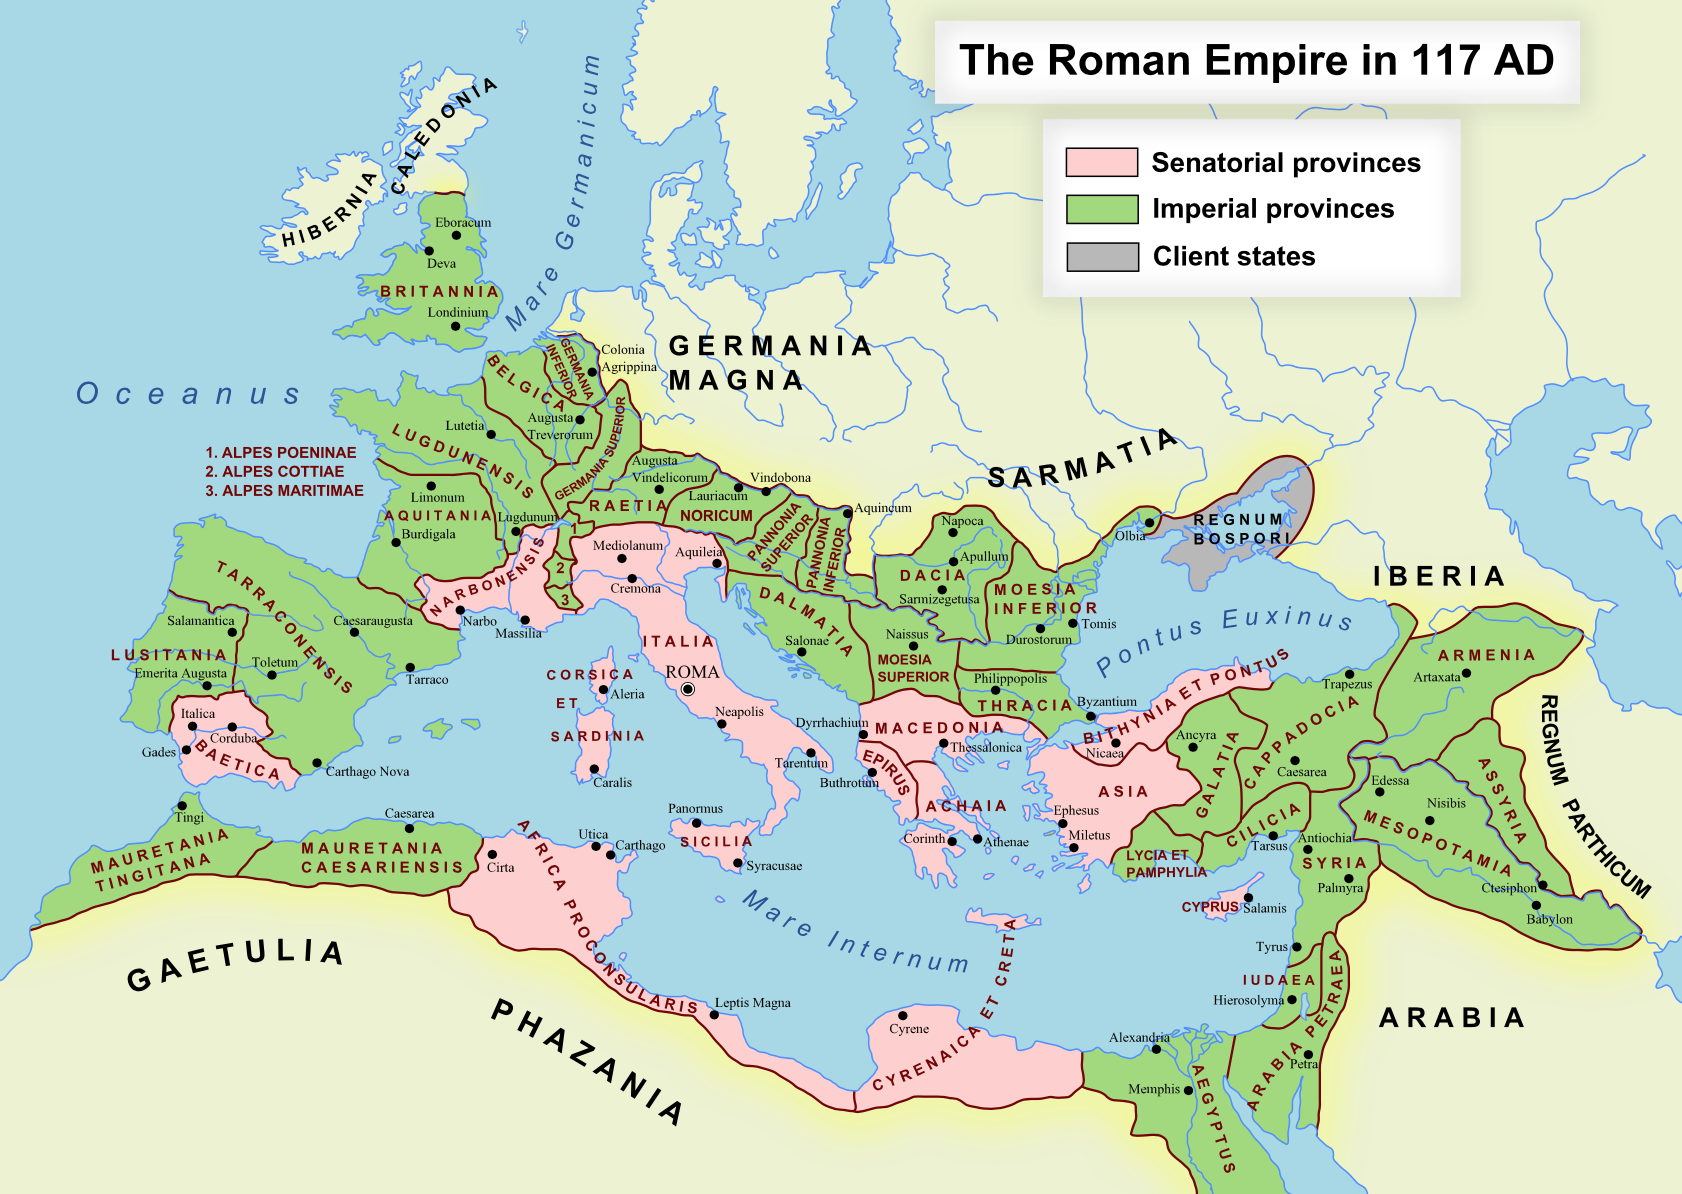
\includegraphics[width=0.95\linewidth]{HMZ5-roman-empire-117.png}
\caption{罗马帝国行省,公元 117 年}
\label{fig:romanempire}
\end{figure}

以下摘录来自《罗马史》第一卷第一、四、五、六、七章和第三卷第八、九、十、十一章,肖婷译。
